\chapter{Intel SGX}
\label{chapter:sgx}

Nesse capítulo é detalhada a tecnologia Intel SGX. Primeiramente, são
introduzidos os principais objetivos da tecnologia. Depois, é definido o modelo
de ameaça considerado pela tecnologia. Em seguida, são apresentados alguns
conceitos envolvidos no entendimento de seu funcionamento. Mais à frente, são
considerados possíveis casos de uso para a tecnologia, e são apresentadas as
principais limitações do SGX. Por fim, são feitas algumas considerações gerais
sobre a tecnologia.

\section{Introdução ao SGX}
\label{sec:sgx_intro}

Intel SGX é uma tecnologia que tem como objetivo implementar um TEE. Ela busca
garantir proteção contra modificação e divulgação de dados e código\footnote{O
código de aplicações é protegido apenas contra modificação.} de aplicações~\cite
{mckeen2013innovative}. Tal proteção é implementada em nível de \textit
{hardware}, onde o processador é responsável pelo controle de acesso a áreas de
memória protegidas criptograficamente -- tentativas de acesso ou modificação não
autorizadas são tratadas como falha ou acesso a uma memória inexistente.

Intel SGX foi inicialmente definida no ano de 2013, e está comercialmente
disponível desde o ano de 2015 em processadores da família Intel Core a partir
da 6\textsuperscript{a} geração, baseados na microarquitetura Skylake, bem como
em alguns processadores Intel Xeon v5.

Ao contrário de tecnologias semelhantes, como ARM TrustZone e AMD SME/SEV, onde
considera-se uma separação única entre um mundo seguro e um mundo inseguro, com
Intel SGX considera-se a existência de um mundo inseguro e vários mundos
seguros, isolados entre si, conhecidos como \textbf{enclaves}.

Desenvolvedores podem proteger as suas aplicações usando SGX, diretamente
através do uso de um conjunto de instruções que foi incorporado às arquiteturas
Intel 64 e IA-32, ou através do uso de um conjunto de APIs e bibliotecas, e um
conjunto de enclaves arquiteturais, conhecidos, respectivamente, por \textit{SGX
SDK} e \textit{SGX PSW}.

\section{Modelo de ameaça}
\label{sec:sgx_modelo_ameaca}

Antes de explicar como Intel SGX alcança os objetivos descritos na seção
anterior, é necessário entender qual o modelo de ameaça considerado pela
tecnologia.
Intel SGX considera um modelo de ameaça onde um atacante é capaz de controlar e
inserir código malicioso em programas com alto nível de privilégio, como
sistemas operacionais e hipervisores, e até mesmo tenha acesso físico ao
\textit{hardware} onde os dados sigilosos se encontram.

Atacantes que consigam controle sobre um sistema operacional ou sobre um monitor
de máquina virtual são capazes de obter e vazar informações sigilosas de
usuários de diversas formas diferentes~\cite{trustshadow2017}.
Já atacantes com acesso físico ao \textit{hardware} podem realizar ataques de
inicialização a frio, e recuperar chaves criptográficas que permanecem na DRAM,
mesmo após a mesma ser removida da placa-mãe \cite{coldbootattack}, e
posteriormente usar essas chaves para obter dados sigilosos sem a devida
autorização.

É importante ressaltar que Intel SGX não oferece proteção contra ataques de
canal lateral~\cite{sgxdeveloperreference}. Vários ataques deste tipo já foram
demonstrados, e provaram ter eficácia contra as proteções providas pelo SGX
isoladamente~\cite{cachezoom2017,gotzfried2017cache,lee2016inferring}. Para
evitar esse tipo de ataque, programadores devem tomar as devidas precauções
~\cite{shinde2015preventing,seo2017sgx,shih2017t}.

\section{Modelo de memória}
\label{sec:sgx_modelo_memoria}

\begin{figure}[ht]
\centering
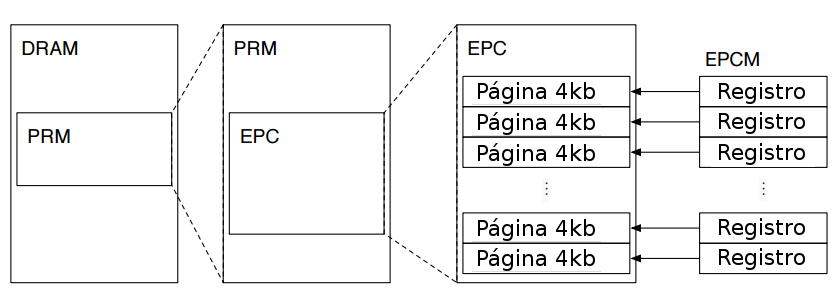
\includegraphics[width=5in]{img/hierarquia_memoria_sgx_pt_BR}
\caption{Hierarquia de memória do Intel SGX}
\label{fig:hierarquiamemoria}
\end{figure}

Intel SGX utiliza uma hierarquia de memória conforme ilustrada na Figura
\ref{fig:hierarquiamemoria}.

Tendo o Intel SGX disponível no processador e habilitado, o BIOS reserva uma
parte da memória principal (DRAM), chamada de \textit{Processor Reserved Memory}
(PRM), e a partir de então o acesso a essa área de memória passa a ser
controlada pelo processador.

Parte da PRM é destinada a uma área de memória conhecida como \textit{Enclave
Page Cache} (EPC). A EPC serve para armazenar páginas de enclaves SGX.
Cada uma dessas páginas é associada a um único enclave SGX. O processador é
responsável por garantir que essas páginas só sejam acessíveis pelo enclave
associado a elas.

Por fim, para auxiliar o controle de acesso à memória, uma estrutura adicional
precisa ser criada. Essa estrutura é conhecida como \textit{Enclave Page Cache
Map} (EPCM), e é utilizada para armazenar metadados -- permissões de leitura,
escrita e execução, tipo, endereço linear, estado, etc. -- sobre as páginas que
residem na EPC.

\subsection{Paginação da EPC}
\label{subsec:sgx_modelo_memoria_paginacao_epc}
De modo a aumentar o número de aplicações protegidas que podem ser suportadas de
forma concorrente, a arquitetura SGX oferece instruções que permitem que
sistemas operacionais façam paginação da EPC de forma segura. O processo de
paginação da EPC também pode ser acionado caso o tamanho dos dados carregados em
um enclave exceda o limite do tamanho da EPC.

O processo de paginação da EPC, em geral, é muito mais custoso que um processo
de paginação normal de um sistema operacional. Isso se deve ao fato de que as
seguintes medidas de segurança devem ser tomadas pelo SGX:

\begin{enumerate}
    \item Uma página de enclave só pode ser removida da EPC depois que todas as
    traduções em cache para essa página tenham sido removidas de todos os
    processadores lógicos;

    \item O conteúdo da página do enclave precisa ser cifrado antes de ser
    escrito na memória principal;

    \item Ao recarregar a página na EPC, informações sobre o tipo, permissões,
    endereço virtual, conteúdo, e o enclave dono da página devem ser
    verificadas, de modo a garantir que as mesmas correspondem à página que foi
    removida;

    \item Apenas a última versão da página removida pode ser recarregada.
\end{enumerate}

\section{Modelo de programação}
\label{sec:sgx_modelo_programacao}

Antes de desenvolver aplicações que fazem uso de Intel SGX, desenvolvedores
devem ter em mente que nem toda a área de sua aplicação deve ser protegida. Na
verdade, a Intel sugere que o mínimo possível da aplicação seja executada dentro
de enclaves SGX -- apenas a parte da aplicação que lida com dados sigilosos.

Dessa forma, aplicações SGX devem ser separadas em duas partes:

\begin{description}
    \item [Parte segura/confiável] -- executada dentro de enclaves SGX. Deve ser
    usada para armazenamento e processamento de dados sensíveis/sigilosos.
    Por ser protegida, há um custo adicional de processamento em comparação com
    a execução de uma aplicação normal, relativo ao processo de cifrar e
    decifrar páginas dos enclaves. Código sendo executado na parte segura não é
    capaz de executar chamadas de sistema.

    \item [Parte insegura/não confiável] -- executada na memória principal da
    máquina. Serve como um invólucro para a parte segura da aplicação, podendo
    ser usado tanto para o processamento de dados que não sejam sigilosos,
    quanto como uma interface de comunicação com outras aplicações ou escrita de
    arquivos.
\end{description}

Para definir como as duas partes da aplicação SGX se comunicam entre si, um
arquivo no formato EDL -- \textit{Enclave Description Language} -- deve ser
provido pelo desenvolvedor. Neste arquivo são definidas funções onde a parte
insegura da aplicação envia dados e executa algum processamento dentro da parte
segura (ECALLs), e funções onde a parte segura da aplicação envia dados e
executa algum processamento na parte insegura (OCalls).

Juntamente com o \textit{SGX SDK} é fornecida uma ferramenta conhecida como
Edger8r. Ela é responsável por ler arquivos EDL e gerar interfaces de
comunicação entre as partes segura e insegura de uma aplicação SGX.

\section{Funcionalidades importantes}
\label{sec:sgx_funcionalidades}

Intel SGX possui algumas funcionalidades que auxiliam no processo de estabelecer
confiança em uma aplicação, bem como no compartilhamento seguro de dados
sigilosos entre diferentes aplicações, ou entre diferentes versões de uma mesma
aplicação. Essas funcionalidades são discutidas a seguir.

\subsection{Medição de enclaves}
\label{subsec:sgx_funcionalidades_medicao_enclaves}

A arquitetura Intel SGX é responsável por estabelecer identidades de enclaves.
No jargão do Intel SGX, o processo de estabelecimento de identidade de um
enclave é conhecido como \textbf{medição de enclave}.
Associadas a cada enclave estão duas identidades distintas:

\begin{description}
    \item [MRENCLAVE] -- Também referido como identidade de enclave, é o
    resultado da função de \textit{hash} SHA-256 do registro de toda a atividade feita ao construir um
    enclave SGX. Em outras palavras, essa identidade é calculada baseada em todo
    o conteúdo carregado em um enclave, \textit{i.e.}, conteúdos das páginas do
    enclave, posição relativa das páginas no enclave, e \textit{flags} de
    segurança associadas às páginas.

    \item [MRSIGNER] -- Também referido como identidade de selagem, é a
    identidade de quem assinou o enclave SGX, tipicamente o desenvolvedor do
    enclave. Múltiplos enclaves podem ser assinados por um mesmo desenvolvedor,
    fazendo com que todos tenham a mesma identidade de selagem.

\end{description}

\subsection{Atestação de enclaves}
\label{subsec:sgx_funcionalidades_atestacao_enclaves}

Atestação é o processo de provar que um determinado programa foi devidamente
instanciado em uma plataforma. No caso do Intel SGX, o processo de atestação
garante que um programa está sendo executado dentro de um enclave SGX, e que não
foram feitas modificações no código do mesmo. O processo de atestação pode ser
feito local ou remotamente.

\subsubsection{Atestação local}
\label{subsubsec:sgx_funcionalidades_atestacao_enclaves_local}

\begin{figure}[ht]
\centering
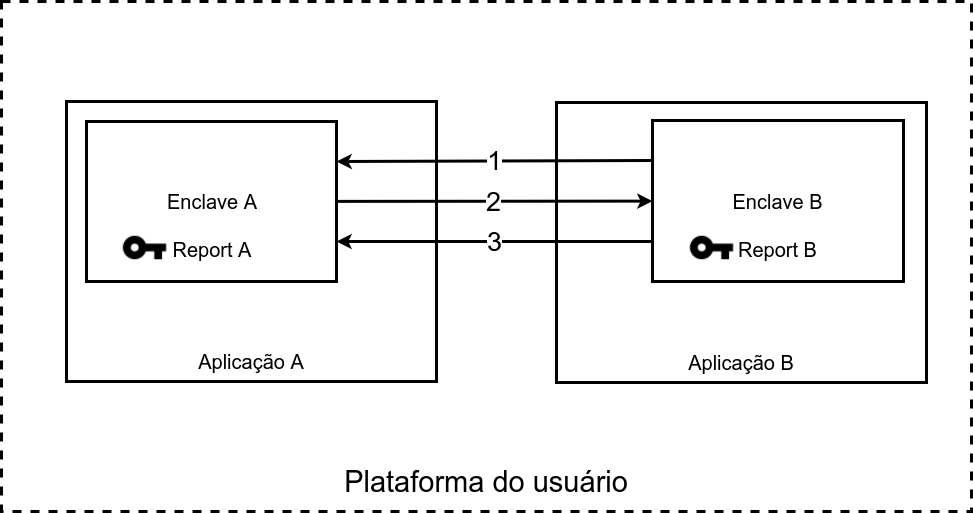
\includegraphics[width=5in]{img/atestacao_local_pt_BR}
\caption{Atestação local}
\label{fig:atestacaolocal}
\end{figure}

Desenvolvedores podem escrever duas ou mais aplicações seguras, executadas em
enclaves, que podem cooperar entre si, para realizar funções que não sejam de
suas próprias competências. Para isso, é provido um mecanismo que permite que
enclaves se autentiquem entre si, através do uso das instruções EREPORT e
EGETKEY.

O processo completo de atestação local de enclaves, ilustrado na Figura
\ref{fig:atestacaolocal}, acontece da seguinte forma:

\begin{enumerate}
    \item Após um canal de comunicação ser estabelecido entre os enclaves A e
    B\footnote{\label{notacomunicacao}Toda comunicação de aplicações SGX passa
    pela parte insegura da aplicação.}, o enclave A obtém o MRENCLAVE do enclave
    B.

    \item O enclave A executa a instrução EREPORT, usando como parâmetro o
    MRENCLAVE do enclave B, criando assim uma estrutura, conhecida como
    \textit{REPORT}, contendo o seu próprio MRENCLAVE e MRSIGNER, e assinada com
    uma chave, \textit{Report Key}, acessível diretamente apenas pelo enclave B.
    Após obtido, o \textit{REPORT} é enviado pelo enclave A para o enclave B.

    \item Tendo recebido o \textit{REPORT} do enclave A:

    \begin{enumerate}
        \item O enclave B executa a instrução EGETKEY para obter a sua chave, e
        com ela, verifica a assinatura do \textit{REPORT} recebido do enclave A.
        Caso a assinatura seja verificada com sucesso, o enclave B pode ter
        certeza que o enclave A está sendo executado na mesma plataforma, que
        por sua vez, está de acordo com o modelo de segurança SGX.

        \item O enclave B pode então verificar se o MRENCLAVE do enclave A,
        contido no \textit{REPORT} recebido, corresponde ao da aplicação com a
        qual ele deseja se comunicar. Em caso positivo, o enclave A pode agora
        ter certeza de estar se comunicando com a aplicação correta.
    \end{enumerate}

\end{enumerate}

O mesmo processo pode ser repetido para que o enclave A confie no enclave B.

\subsubsection{Atestação remota}
\label{subsubsec:sgx_funcionalidades_atestacao_enclaves_remota}

\begin{figure}[ht]
\centering
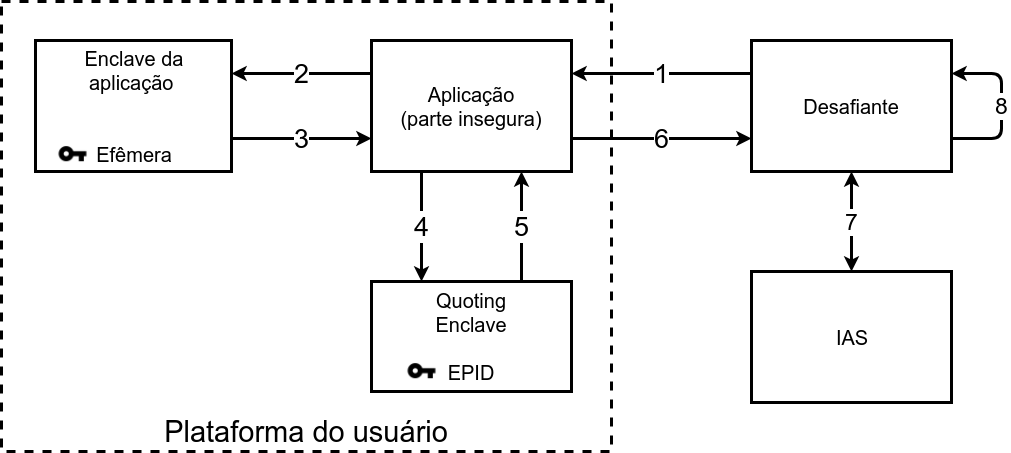
\includegraphics[width=5in]{img/atestacao_remota_pt_BR}
\caption{Atestação remota}
\label{fig:atestacaoremota}
\end{figure}

O processo de atestação local usa um sistema de chaves simétricas, onde a chave
só é acessível através da execução das instruções \textit{EREPORT} e \textit{
EGETKEY}. No caso de uma atestação remota (RA, do inglês \textit{Remote
Attestation}), a aplicação que deseja ganhar confiança em uma aplicação SGX não
é capaz de executar a instrução \textit{EGETKEY}, uma vez que as partes são
executadas em plataformas distintas. Para o processo de atestação remota, é
necessário o uso de um sistema de chaves assimétricas.

Para permitir tal processo, um enclave especial, conhecido como \textit{Quoting
Enclave} (QE), é provido pela Intel. O QE é responsável por usar o processo de
atestação local, e transformar o \textit{REPORT} gerado no processo em uma outra
estrutura, conhecida como \textit{QUOTE}, assinada com uma chave assimétrica,
acessível apenas pelo QE.
Além disso, a Intel provê um serviço de atestação (IAS), que é capaz de
verificar a autenticidade da assinatura de um \textit{QUOTE}.

O processo completo de atestação remota, mostrado na Figura
\ref{fig:atestacaoremota}, acontece da seguinte forma:

\begin{enumerate}
    \item Após estabelecida uma comunicação entre um desafiante e a plataforma
    onde se encontra a aplicação SGX\footref{notacomunicacao}, o desafiante pede
    uma prova de que a aplicação está sendo devidamente executada dentro de um
    enclave SGX. Junto a esse pedido, o desafiante envia a sua chave pública.

    \item Recebendo tal pedido, o enclave procede criando uma estrutura,
    \textit{MSG1}, que contém sua chave pública, e a envia para o desafiante.

    \item Em seguida, o desafiante é capaz de derivar uma chave
    simétrica, \textit{SMK}, através do método \textit{Diffie-Hellman}, usando a
    sua chave privada e a chave pública do enclave. Tendo essa chave simétrica
    em mãos, o desafiante deve gerar uma outra estrutura, \textit{MSG2}, e
    enviar para o enclave. A \textit{MSG2} contém:
    \begin{enumerate}
        \item a chave pública do desafiante;
        \item um identificador de registro do desafiante para com o IAS;
        \item uma assinatura da concatenação de ambas as chaves públicas, usando
        a chave privada do desafiante;
        \item um código de autenticação de mensagem (MAC) de toda a mensagem,
        usando a chave \textit{SMK}, que pode ser verificada pelo enclave.
    \end{enumerate}

    \item O enclave deve então gerar o seu \textit{REPORT}, e enviar para o QE,
    para que ele gere o \textit{QUOTE} do enclave.

    \item O enclave gera um \textit{MAC} do \textit{QUOTE} recebido, usando a
    chave \textit{SMK}, e a envia para o desafiante.

    \item O desafiante verifica o \textit{MAC}, para garantir que está se
    comunicando com o mesmo enclave ainda, e após verificar com sucesso, envia o
    \textit{QUOTE} para o \textit{IAS}.

    \item O \textit{IAS} verifica se a assinatura e a estrutura do \textit{QUOTE}
    são válidos, ou seja, foram gerados por um enclave SGX, e envia um resposta
    para o desafiante.

    \item Tendo confirmado a validade do \textit{QUOTE}, o desafiante verifica
    se o \textit{MRENCLAVE}, contido no \textit{QUOTE}, é o esperado,
    completando assim o processo de atestação remota.

\end{enumerate}

Após completar o processo de atestação remota, ambas as partes envolvidas podem
usar a chave \textit{SMK} para enviar mensagens entre si de forma segura.

\subsection{Selagem de dados}
\label{subsec:sgx_funcionalidades_selagem_dados}

Enquanto um enclave está instanciado, o \textit{hardware} garante a integridade
e confidencialidade de seus dados. Entretanto, ao encerrar o processo de um
enclave, todo o seu conteúdo é destruído, e qualquer dado que esteja no enclave
será perdido.

Se os dados do enclave seriam usados posteriormente, \textit{e.g.}, em uma
futura execução do enclave, é necessário que esses dados sejam armazenados fora
da área protegida do enclave.
Com este objetivo, o SGX provê uma funcionalidade para selar estes dados e
armazená-los em disco de forma segura.
A funcionalidade de selagem de dados pode ser feita de duas formas:

\begin{description}
    \item [Selagem usando a Identidade de enclave] -- Utilizada quando apenas o
    mesmo código de enclave deve ser capaz de acessar os dados selados. Utiliza
    o MRENCLAVE para selar os dados.
    Com essa forma de selagem, não é possível transferir dados para aplicações
    diferentes, ou até mesmo para uma nova versão da mesma aplicação.

    \item [Selagem usando a Identidade de selagem] -- Utilizada quando se deseja
    transferir dados de um enclave para uma aplicação distinta ou para uma nova
    versão da mesma aplicação. Utiliza o MRSIGNER para selar os dados.
    Os dados selados serão acessíveis por qualquer enclave que tenha sido
    assinado pelo mesmo desenvolvedor, o que resulta em um mesmo MRENCLAVE.
    Também é útil quando se deseja atualizar uma aplicação, \textit{e.g.},
    quando deseja-se usar um código mais eficiente ou mais seguro na aplicação.
\end{description}

\section{Ciclo de vida de aplicações SGX}
\label{sec:sgx_ciclo_vida}

\begin{figure}[ht]
\centering
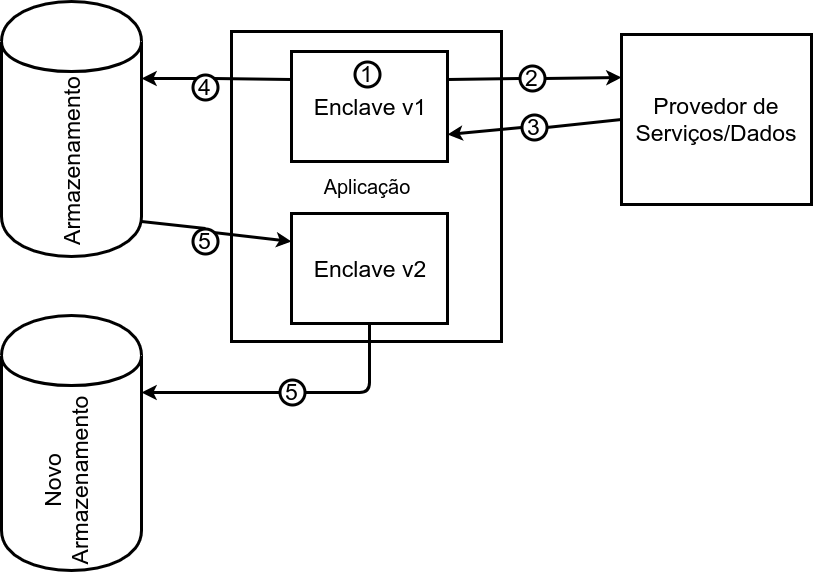
\includegraphics[width=5in]{img/ciclovida_sgx}
\caption{Ciclo de vida de aplicações SGX}
\label{fig:ciclovida}
\end{figure}

Aplicações SGX devem ser iniciadas sem conter nenhum dado sigiloso na memória.
Depois que o enclave SGX já está sendo executado, o processo de atestação de
enclaves pode ser usado para obter confiança em uma aplicação SGX, e estabelecer
um canal de comunicação seguro, para enviar dados para serem processados dentro
do enclave da aplicação SGX.

A aplicação SGX pode cifrar os seus dados e armazená-los para um uso futuro,
usando a funcionalidade de selagem de dados.

A Figura \ref{fig:ciclovida} ilustra os passos dados para completar esse ciclo.

\begin{enumerate}
    \item Inicialização de enclave -- A parte insegura da aplicação é
    responsável por criar o enclave. No processo de inicialização do enclave o
    seu MRENCLAVE é calculado.

    \item Atestação -- A aplicação SGX usa o processo de atestação remota para
    se tornar confiável e estabelecer um canal de comunicação seguro.

    \item Provisionamento -- A aplicação SGX recebe os dados sigilosos através
    do canal de comunicação seguro.

    \item Selagem -- O enclave usa a funcionalidade de selagem para armazenar
    seus dados sigilosos de forma que uma nova versão da aplicação possa
    acessá-los.

    \item Atualização de aplicação -- Uma aplicação SGX pode necessitar de uma
    atualização, e sua versão atualizada recebe os dados da versão anterior.

\end{enumerate}

\section{Intel SGX SDK e PSW}
\label{sec:sgx_sdk_psw}

O SDK é um conjunto de ferramentas e APIs com funções de alto nível (em C/C++)
que permite a criação e uso de enclaves SGX de forma mais fácil para o
desenvolvedor.
Juntamente com o SDK estão presentes duas ferramentas essenciais no ciclo de
vida de aplicações SGX. São elas:

\begin{itemize}
    \item sgx\_edger8r -- responsável por criar as interfaces de comunicação
    entre as partes segura e insegura da aplicação.

    \item sgx\_sign -- responsável por assinar um enclave SGX, usando uma chave
    privada, que resultará no MRSIGNER do enclave.
\end{itemize}

Já o PSW, distribuído junto do SDK, trata-se de um conjunto de enclaves especias
da Intel, usados para instanciar e realizar o processo de medição enclaves.
Entre os enclaves mais importantes estão:

\begin{itemize}
    \item \textit{Launch Enclave} (LE) -- responsável por instanciar enclaves
    SGX.

    \item \textit{Quoting Enclave} (QE) -- responsável por gerar a estrutura
    conhecida como QUOTE, usada no processo de atestação remota de enclaves SGX.

    \item \textit{Provisioning enclave} (PvE) -- responsável por prover chaves
    necessárias ao processo de atestação de um enclave.
\end{itemize}

Ambos o SDK e o PSW estão disponíveis tanto para a plataforma \textit{Windows}
quanto para a plataforma \textit{Linux}\footnote{\label{fn:SGXSDK}\url
{https://software.intel.com/en-us/sgx-sdk/download}}.

\section{Casos de uso de SGX}
\label{sec:sgx_casos_de_uso}

Considerando aplicações do tipo cliente-servidor que usam SGX, podemos observar
dois modelos: ($i$) proteção de dados no lado do cliente, ou ($ii$) proteção de
dados no lado do servidor.

\subsection*{Máquina cliente como \textit{host} do enclave SGX}

Neste modelo de aplicação, o objetivo é ter uma aplicação na máquina cliente que
\textbf{obtém} dados sensíveis de algum provedor de serviços. Antes de receber
tais dados, a aplicação precisa provar para o provedor de serviços que está
sendo executada em um enclave SGX.

Como exemplo de aplicação que pode tirar proveito de SGX para proteção de dados
sigilosos, podemos citar uma aplicação de \textit{Internet Banking}. Neste caso,
a entidade financeira em posse dos dados de um cliente precisa se certificar que
os dados sensíveis, \textit{e.g.}, saldo e extrato de conta, só serão acessíveis
pelo cliente a quem a conta pertence. Para alcançar este objetivo, a entidade
financeira pode desenvolver uma aplicação que execute dentro de um enclave SGX,
e que seja atestável pelo seu provedor de serviços.

Outro caso de uso deste modelo que podemos citar é o de gestão de direitos
digitais (DRM, do inglês \textit{Digital Rights Management}). Neste caso, um
enclave SGX pode ser utilizado para evitar que cópias de conteúdos digitais
sejam feitas sem a devida autorização. Uma grande empresa que atualmente está
utilizando Intel SGX para este fim é a Netflix\footnote{\url
{https://help.netflix.com/pt/node/55763}}. Ela utiliza as capacidades do SGX
para proteger vídeos transmitidos com qualidade 4K.

\subsection*{Máquina servidora como \textit{host} do enclave SGX}

Neste modelo de aplicação, o objetivo é ter uma aplicação na máquina cliente que
\textbf{envia} dados sensíveis para algum provedor de serviços. Antes de enviar
tais dados, a aplicação precisa ter certeza que está se comunicando com um
provedor de dados confiável, \textit{i.e.}, está executando em um enclave SGX.

Um caso de uso que podemos citar como exemplo deste modelo é o de agregação de
dados de \textit{smart meters}~\cite{sac2017}. Neste caso, \textit{smart meters}
coletam dados de consumo de energia de residências com um alto nível de detalhe.
Estes dados podem ser usados para derivar informações sobre os indivíduos que
ali residem\footnote{\url{https://www.cnet.com/news/researchers-find-smart-
meters-could-reveal-favorite-tv-shows/}}. Desta forma, é necessário prover um
certo nível de proteção destes dados, para que eles só possam ser utilizados
de forma agregada por distribuidores de energia.

\section{Limitações do Intel SGX}
\label{sec:sgx_limitacoes}

Como qualquer outra tecnologia, Intel SGX também possui limitações. As mais
importantes delas são discutidas a seguir.

\subsection{Privacidade de código}
\label{subsec:sgx_limitacoes_privacidade_codigo}

Apesar de dar garantias quanto à proteção do código de aplicações contra
modificações não autorizadas, Intel SGX não garante a privacidade desse mesmo
código. Em outras palavras, arquivos contendo todo o código de um enclave SGX
são carregados na memória principal de forma não cifrada.

Há vários cenários onde desenvolvedores desejam manter a privacidade de seu
código, portanto essa limitação deve ser levada em consideração por
desenvolvedores, uma vez que atacantes poderiam facilmente usar ferramentas como
o IDA \cite{idapro} para gerar um pseudo-código bastante similar à aplicação
original.

\subsection{Ligação estática de bibliotecas}
\label{subsec:sgx_limitacoes_ligacao_estatica}

Aplicações que usam bibliotecas de terceiros precisam ligar tais bibliotecas a
seus enclaves estaticamente. Isso pode resultar em um enclave demasiadamente
grande, e, consequentemente desperdiçar espaço da memória, que é um recurso
bastante escaço para o SGX. Outra consequência desta limitação é que qualquer
mínima modificação em uma única biblioteca pela aplicação requer que toda a
aplicação SGX seja completamente recompilada e reimplantada.

\subsection{Memória disponível}
\label{subsec:sgx_limitacoes_memoria}

O espaço da memória principal usado pela PRM deve ser reservado pelo BIOS no
momento em que o sistema está sendo inicializado. Além disso, toda a EPC deve
residir dentro da PRM. Na versão atual do SGX, a parte da memória reservada para
a PRM é limitada a um tamanho máximo de apenas $128\ MB$ por máquina. Caso o espaço
necessário seja maior do que o disponível, há um grande aumento no tempo de
processamento, devido ao custoso processo de paginação entre EPC e DRAM,
conforme descrito na seção~\ref{subsec:sgx_modelo_memoria_paginacao_epc}. Na
seção~\ref{sec:abordagem_gerencia_memoria} discutiremos melhor os impactos da
gerência de memória protegida.

\subsection{Vulnerabilidades}
\label{subsec:sgx_limitacoes_vulnerabilidades}

Conforme descrito na Seção~\ref{sec:sgx_modelo_ameaca}, aplicações SGX podem ser
vulneráveis a ataques de canal lateral. Esse tipo de ataque permite que um
adversário colete estatísticas sobre execução da \textbf{CPU}, e as utilize para
deduzir características sobre o programa em execução. Apesar de SGX não prover
proteção contra esse tipo de ataque, é possível previní-lo, tomando os devidos
cuidados\footnote{\url
{https://github.com/chowes/sgx-side-channel/blob/master/sgx-side-channel.pdf}}.

É importante notarmos também que a solução de SGX é composta por componentes --
\textit{drivers}, bibliotecas, e instruções -- complexos, e, portanto,
dificilmente é completamente livre de erros, como qualquer outro
\textit{software}. Além disso, desenvolvedores de aplicações SGX podem cometer
erros e escrever enclaves suscetíveis a vulnerabilidades como \textit
{buffer overflow} e formatação não verificada de \textit{strings}.

Uma técnica de segurança que tem suas funcionalidades limitadas com o uso de SGX
é a de aleatorização do leiaute do espaço de endereçamento (ASLR, do inglês
\textit{Address Space Layout Randomization}). Esta técnica torna aleatória a
organização na memória de diversas partes de um processo, evitando assim que
atacantes usem as vulnerabilidades mencionadas anteriormente para desviar a
execução de um programa para uma função explorada carregada na memória. No
caso do SGX, por ter um espaço de endereçamento reduzido, ataques de força bruta
podem ser utilizados para descobrir o endereço desejado. Em experimentos
realizados, foi verificado que em diferentes execuções, uma variável de um
enclave SGX tem seu endereço modificado em apenas dois \textit{bytes},
significando que a aleatorização tem aproximadamente apenas $65536$
possibilidades. Essa quantidade de possibilidades é muito pequena, uma vez que
atacantes podem aumentar a probabilidade de ataques com sucesso através da
injeção de sequências de instruções \textbf{NOP} antes de um código malicioso.

\section{Considerações}

Intel SGX é uma tecnologia bastante promissora, oferecendo garantias de
segurança e privacidade de dados de usuários contra ataques provenientes até
mesmo de atacantes que tenham obtido privilégio indevidamente, ou que tenham
acesso físico à máquina que hospeda os dados sigilosos. Como qualquer outra
tecnologia, porém, também possui limitações que podem pôr em risco a sua
aplicabilidade no mundo real. É necessário, portanto, fazer uma análise dos
principais desafios a serem enfrentados durante o processo de desenvolvimento de
aplicações que façam uso desta tecnologia, antes de pô-la em um ambiente de
produção.